\documentclass[twoside]{book}

% Packages required by doxygen
\usepackage{fixltx2e}
\usepackage{calc}
\usepackage{doxygen}
\usepackage[export]{adjustbox} % also loads graphicx
\usepackage{graphicx}
\usepackage[utf8]{inputenc}
\usepackage{makeidx}
\usepackage{multicol}
\usepackage{multirow}
\PassOptionsToPackage{warn}{textcomp}
\usepackage{textcomp}
\usepackage[nointegrals]{wasysym}
\usepackage[table]{xcolor}

% Font selection
\usepackage[T1]{fontenc}
\usepackage[scaled=.90]{helvet}
\usepackage{courier}
\usepackage{amssymb}
\usepackage{sectsty}
\renewcommand{\familydefault}{\sfdefault}
\allsectionsfont{%
  \fontseries{bc}\selectfont%
  \color{darkgray}%
}
\renewcommand{\DoxyLabelFont}{%
  \fontseries{bc}\selectfont%
  \color{darkgray}%
}
\newcommand{\+}{\discretionary{\mbox{\scriptsize$\hookleftarrow$}}{}{}}

% Page & text layout
\usepackage{geometry}
\geometry{%
  a4paper,%
  top=2.5cm,%
  bottom=2.5cm,%
  left=2.5cm,%
  right=2.5cm%
}
\tolerance=750
\hfuzz=15pt
\hbadness=750
\setlength{\emergencystretch}{15pt}
\setlength{\parindent}{0cm}
\setlength{\parskip}{3ex plus 2ex minus 2ex}
\makeatletter
\renewcommand{\paragraph}{%
  \@startsection{paragraph}{4}{0ex}{-1.0ex}{1.0ex}{%
    \normalfont\normalsize\bfseries\SS@parafont%
  }%
}
\renewcommand{\subparagraph}{%
  \@startsection{subparagraph}{5}{0ex}{-1.0ex}{1.0ex}{%
    \normalfont\normalsize\bfseries\SS@subparafont%
  }%
}
\makeatother

% Headers & footers
\usepackage{fancyhdr}
\pagestyle{fancyplain}
\fancyhead[LE]{\fancyplain{}{\bfseries\thepage}}
\fancyhead[CE]{\fancyplain{}{}}
\fancyhead[RE]{\fancyplain{}{\bfseries\leftmark}}
\fancyhead[LO]{\fancyplain{}{\bfseries\rightmark}}
\fancyhead[CO]{\fancyplain{}{}}
\fancyhead[RO]{\fancyplain{}{\bfseries\thepage}}
\fancyfoot[LE]{\fancyplain{}{}}
\fancyfoot[CE]{\fancyplain{}{}}
\fancyfoot[RE]{\fancyplain{}{\bfseries\scriptsize Generated by Doxygen }}
\fancyfoot[LO]{\fancyplain{}{\bfseries\scriptsize Generated by Doxygen }}
\fancyfoot[CO]{\fancyplain{}{}}
\fancyfoot[RO]{\fancyplain{}{}}
\renewcommand{\footrulewidth}{0.4pt}
\renewcommand{\chaptermark}[1]{%
  \markboth{#1}{}%
}
\renewcommand{\sectionmark}[1]{%
  \markright{\thesection\ #1}%
}

% Indices & bibliography
\usepackage{natbib}
\usepackage[titles]{tocloft}
\setcounter{tocdepth}{3}
\setcounter{secnumdepth}{5}
\makeindex

% Hyperlinks (required, but should be loaded last)
\usepackage{ifpdf}
\ifpdf
  \usepackage[pdftex,pagebackref=true]{hyperref}
\else
  \usepackage[ps2pdf,pagebackref=true]{hyperref}
\fi
\hypersetup{%
  colorlinks=true,%
  linkcolor=blue,%
  citecolor=blue,%
  unicode%
}

% Custom commands
\newcommand{\clearemptydoublepage}{%
  \newpage{\pagestyle{empty}\cleardoublepage}%
}

\usepackage{caption}
\captionsetup{labelsep=space,justification=centering,font={bf},singlelinecheck=off,skip=4pt,position=top}

%===== C O N T E N T S =====

\begin{document}

% Titlepage & ToC
\hypersetup{pageanchor=false,
             bookmarksnumbered=true,
             pdfencoding=unicode
            }
\pagenumbering{alph}
\begin{titlepage}
\vspace*{7cm}
\begin{center}%
{\Large FB Render\+Lib \\[1ex]\large 1.\+0.\+0 }\\
\vspace*{1cm}
{\large Generated by Doxygen 1.8.13}\\
\end{center}
\end{titlepage}
\clearemptydoublepage
\pagenumbering{roman}
\tableofcontents
\clearemptydoublepage
\pagenumbering{arabic}
\hypersetup{pageanchor=true}

%--- Begin generated contents ---
\chapter{Hierarchical Index}
\section{Class Hierarchy}
This inheritance list is sorted roughly, but not completely, alphabetically\+:\begin{DoxyCompactList}
\item \contentsline{section}{Game\+Time}{\pageref{class_game_time}}{}
\item \contentsline{section}{Material}{\pageref{class_material}}{}
\item \contentsline{section}{Mesh}{\pageref{class_mesh}}{}
\item \contentsline{section}{Node\+Component}{\pageref{class_node_component}}{}
\item \contentsline{section}{Render\+Command}{\pageref{class_render_command}}{}
\item \contentsline{section}{Render\+Device}{\pageref{class_render_device}}{}
\item \contentsline{section}{Scene}{\pageref{class_scene}}{}
\begin{DoxyCompactList}
\item \contentsline{section}{Default\+Scene}{\pageref{class_default_scene}}{}
\end{DoxyCompactList}
\item \contentsline{section}{Scene\+Node}{\pageref{class_scene_node}}{}
\item \contentsline{section}{Texture}{\pageref{class_texture}}{}
\end{DoxyCompactList}

\chapter{Class Index}
\section{Class List}
Here are the classes, structs, unions and interfaces with brief descriptions\+:\begin{DoxyCompactList}
\item\contentsline{section}{\hyperlink{class_default_scene}{Default\+Scene} \\*The \hyperlink{class_default_scene}{Default\+Scene} is a simple \hyperlink{class_scene}{Scene} implementation based on a simple vector of Scene\+Nodes. No culling optimization is implemented }{\pageref{class_default_scene}}{}
\item\contentsline{section}{\hyperlink{class_game_time}{Game\+Time} \\*This class contains different kinds of time information, such as the total time the game is running, the last frametime etc }{\pageref{class_game_time}}{}
\item\contentsline{section}{\hyperlink{class_material}{Material} }{\pageref{class_material}}{}
\item\contentsline{section}{\hyperlink{class_mesh}{Mesh} }{\pageref{class_mesh}}{}
\item\contentsline{section}{\hyperlink{class_node_component}{Node\+Component} \\*A \hyperlink{class_node_component}{Node\+Component} is a modular building block of Scene\+Nodes. It has an execute method which can run arbitrary logic. As of now, there is no option to render from a component }{\pageref{class_node_component}}{}
\item\contentsline{section}{\hyperlink{class_render_command}{Render\+Command} \\*This class stores the information to render a specific mesh with a texture and a material }{\pageref{class_render_command}}{}
\item\contentsline{section}{\hyperlink{class_render_device}{Render\+Device} \\*This class takes care of the low level rendering functionality }{\pageref{class_render_device}}{}
\item\contentsline{section}{\hyperlink{class_scene}{Scene} \\*A \hyperlink{class_scene}{Scene} object is the heart of the rendering in the FB renderlib. It consists of Scene\+Nodes which are the foundational objects to be rendered and the user interacts with }{\pageref{class_scene}}{}
\item\contentsline{section}{\hyperlink{class_scene_node}{Scene\+Node} \\*A \hyperlink{class_scene_node}{Scene\+Node} is the main building block of a scene and represents the \char`\"{}game objects\char`\"{} of a game. Each \hyperlink{class_scene_node}{Scene\+Node} has a location and rotation in the world, and can update and render itself during a frame of execution }{\pageref{class_scene_node}}{}
\item\contentsline{section}{\hyperlink{class_texture}{Texture} }{\pageref{class_texture}}{}
\end{DoxyCompactList}

\chapter{Class Documentation}
\hypertarget{class_default_scene}{}\section{Default\+Scene Class Reference}
\label{class_default_scene}\index{Default\+Scene@{Default\+Scene}}


The \hyperlink{class_default_scene}{Default\+Scene} is a simple \hyperlink{class_scene}{Scene} implementation based on a simple vector of Scene\+Nodes. No culling optimization is implemented.  




{\ttfamily \#include $<$scene.\+h$>$}

Inheritance diagram for Default\+Scene\+:\begin{figure}[H]
\begin{center}
\leavevmode
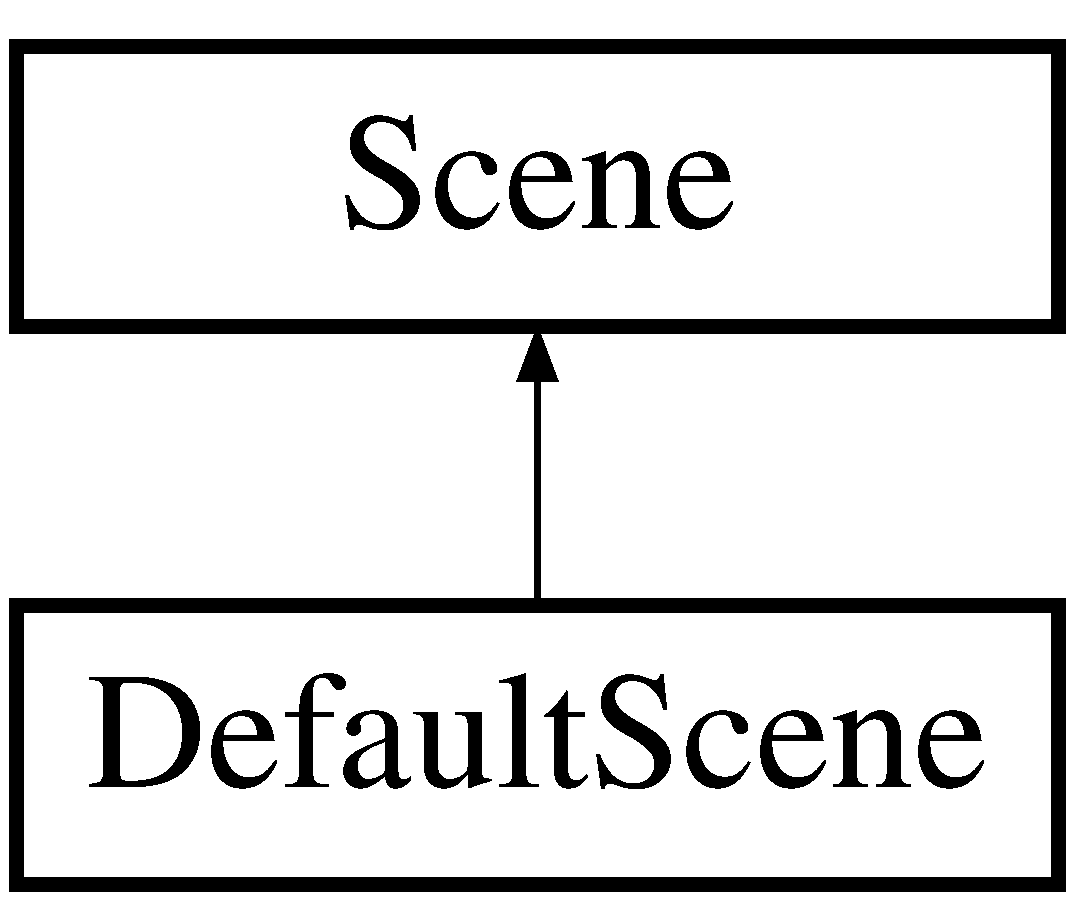
\includegraphics[height=2.000000cm]{class_default_scene}
\end{center}
\end{figure}
\subsection*{Public Member Functions}
\begin{DoxyCompactItemize}
\item 
\mbox{\Hypertarget{class_default_scene_a4b1d299c3da3a3e1b1bff200c2318817}\label{class_default_scene_a4b1d299c3da3a3e1b1bff200c2318817}} 
{\bfseries Default\+Scene} (const \hyperlink{class_default_scene}{Default\+Scene} \&other)=delete
\item 
\mbox{\Hypertarget{class_default_scene_aee5e01122ca501009367babfffbd7a98}\label{class_default_scene_aee5e01122ca501009367babfffbd7a98}} 
\hyperlink{class_default_scene}{Default\+Scene} \& {\bfseries operator=} (\hyperlink{class_default_scene}{Default\+Scene} \&other)=delete
\item 
\mbox{\Hypertarget{class_default_scene_a0de40100cc0236f656cdaf80d5ff477f}\label{class_default_scene_a0de40100cc0236f656cdaf80d5ff477f}} 
virtual R\+E\+N\+D\+E\+R\+L\+I\+B\+\_\+\+A\+PI void \hyperlink{class_default_scene_a0de40100cc0236f656cdaf80d5ff477f}{add\+Node} (std\+::unique\+\_\+ptr$<$ \hyperlink{class_scene_node}{Scene\+Node} $>$ node) override
\begin{DoxyCompactList}\small\item\em Adds a node to the scene graph. \end{DoxyCompactList}\item 
\mbox{\Hypertarget{class_default_scene_a879ed798a8efe945ffb3624f5692e15b}\label{class_default_scene_a879ed798a8efe945ffb3624f5692e15b}} 
virtual R\+E\+N\+D\+E\+R\+L\+I\+B\+\_\+\+A\+PI void \hyperlink{class_default_scene_a879ed798a8efe945ffb3624f5692e15b}{remove\+Node} (const std\+::string \&node\+Id) override
\begin{DoxyCompactList}\small\item\em Removes a node from the scenegraph, destroying it effectively. \end{DoxyCompactList}\item 
\mbox{\Hypertarget{class_default_scene_afb05291c5c6acae4c29abffe8ea30136}\label{class_default_scene_afb05291c5c6acae4c29abffe8ea30136}} 
virtual R\+E\+N\+D\+E\+R\+L\+I\+B\+\_\+\+A\+PI void \hyperlink{class_default_scene_afb05291c5c6acae4c29abffe8ea30136}{update} () override
\begin{DoxyCompactList}\small\item\em Updates the complete scene, gives all nodes a chance to update. \end{DoxyCompactList}\item 
\mbox{\Hypertarget{class_default_scene_a403105049cb05f5f1144e029cd915297}\label{class_default_scene_a403105049cb05f5f1144e029cd915297}} 
virtual R\+E\+N\+D\+E\+R\+L\+I\+B\+\_\+\+A\+PI void \hyperlink{class_default_scene_a403105049cb05f5f1144e029cd915297}{render} (\hyperlink{class_render_device}{Render\+Device} \&render\+Device) override
\begin{DoxyCompactList}\small\item\em Renders the complete scene. \end{DoxyCompactList}\end{DoxyCompactItemize}


\subsection{Detailed Description}
The \hyperlink{class_default_scene}{Default\+Scene} is a simple \hyperlink{class_scene}{Scene} implementation based on a simple vector of Scene\+Nodes. No culling optimization is implemented. 

The documentation for this class was generated from the following files\+:\begin{DoxyCompactItemize}
\item 
C\+:/\+Users/martin/\+Documents/\+Visual Studio 2013/\+Projects/glfw\+\_\+test/\+Render\+Lib/scene.\+h\item 
C\+:/\+Users/martin/\+Documents/\+Visual Studio 2013/\+Projects/glfw\+\_\+test/\+Render\+Lib/scene.\+cpp\end{DoxyCompactItemize}

\hypertarget{class_game_time}{}\section{Game\+Time Class Reference}
\label{class_game_time}\index{Game\+Time@{Game\+Time}}


This class contains different kinds of time information, such as the total time the game is running, the last frametime etc.  




{\ttfamily \#include $<$gametime.\+h$>$}

\subsection*{Public Member Functions}
\begin{DoxyCompactItemize}
\item 
\mbox{\Hypertarget{class_game_time_ac95dfc025f3d267486029edd1d57f9be}\label{class_game_time_ac95dfc025f3d267486029edd1d57f9be}} 
virtual long \hyperlink{class_game_time_ac95dfc025f3d267486029edd1d57f9be}{get\+Total\+Game\+Time} ()
\begin{DoxyCompactList}\small\item\em returns the time the game is running, in ms \end{DoxyCompactList}\item 
\mbox{\Hypertarget{class_game_time_a02a9beaaa0b5ea0ea0619a275996239b}\label{class_game_time_a02a9beaaa0b5ea0ea0619a275996239b}} 
virtual long \hyperlink{class_game_time_a02a9beaaa0b5ea0ea0619a275996239b}{get\+Frame\+Time} ()
\begin{DoxyCompactList}\small\item\em returns the last frame duration in ms \end{DoxyCompactList}\end{DoxyCompactItemize}


\subsection{Detailed Description}
This class contains different kinds of time information, such as the total time the game is running, the last frametime etc. 

The documentation for this class was generated from the following files\+:\begin{DoxyCompactItemize}
\item 
C\+:/\+Users/martin/\+Documents/\+Visual Studio 2013/\+Projects/glfw\+\_\+test/\+Render\+Lib/gametime.\+h\item 
C\+:/\+Users/martin/\+Documents/\+Visual Studio 2013/\+Projects/glfw\+\_\+test/\+Render\+Lib/gametime.\+cpp\end{DoxyCompactItemize}

\hypertarget{class_material}{}\section{Material Class Reference}
\label{class_material}\index{Material@{Material}}


The documentation for this class was generated from the following file\+:\begin{DoxyCompactItemize}
\item 
C\+:/\+Users/martin/\+Documents/\+Visual Studio 2013/\+Projects/glfw\+\_\+test/\+Render\+Lib/material.\+h\end{DoxyCompactItemize}

\hypertarget{class_mesh}{}\section{Mesh Class Reference}
\label{class_mesh}\index{Mesh@{Mesh}}


The documentation for this class was generated from the following file\+:\begin{DoxyCompactItemize}
\item 
C\+:/\+Users/martin/\+Documents/\+Visual Studio 2013/\+Projects/glfw\+\_\+test/\+Render\+Lib/mesh.\+h\end{DoxyCompactItemize}

\hypertarget{class_node_component}{}\section{Node\+Component Class Reference}
\label{class_node_component}\index{Node\+Component@{Node\+Component}}


A \hyperlink{class_node_component}{Node\+Component} is a modular building block of Scene\+Nodes. It has an execute method which can run arbitrary logic. As of now, there is no option to render from a component.  




{\ttfamily \#include $<$nodecomponent.\+h$>$}

\subsection*{Public Member Functions}
\begin{DoxyCompactItemize}
\item 
\mbox{\Hypertarget{class_node_component_a3a3a569f380b8f8e52252b1a4c8ceccf}\label{class_node_component_a3a3a569f380b8f8e52252b1a4c8ceccf}} 
virtual void \hyperlink{class_node_component_a3a3a569f380b8f8e52252b1a4c8ceccf}{execute} ()=0
\begin{DoxyCompactList}\small\item\em This method is called each frame when the owning Scene\+Nodes update method is run. \end{DoxyCompactList}\item 
\mbox{\Hypertarget{class_node_component_a389e825b338a11798186848ce972c62f}\label{class_node_component_a389e825b338a11798186848ce972c62f}} 
virtual \hyperlink{class_scene_node}{Scene\+Node} \& \hyperlink{class_node_component_a389e825b338a11798186848ce972c62f}{get\+Scene\+Node} ()=0
\begin{DoxyCompactList}\small\item\em Get the parent \hyperlink{class_scene_node}{Scene\+Node} reference of this component. \end{DoxyCompactList}\end{DoxyCompactItemize}


\subsection{Detailed Description}
A \hyperlink{class_node_component}{Node\+Component} is a modular building block of Scene\+Nodes. It has an execute method which can run arbitrary logic. As of now, there is no option to render from a component. 

The documentation for this class was generated from the following file\+:\begin{DoxyCompactItemize}
\item 
C\+:/\+Users/martin/\+Documents/\+Visual Studio 2013/\+Projects/glfw\+\_\+test/\+Render\+Lib/nodecomponent.\+h\end{DoxyCompactItemize}

\hypertarget{class_render_command}{}\section{Render\+Command Class Reference}
\label{class_render_command}\index{Render\+Command@{Render\+Command}}


This class stores the information to render a specific mesh with a texture and a material.  




{\ttfamily \#include $<$rendercommand.\+h$>$}

\subsection*{Public Member Functions}
\begin{DoxyCompactItemize}
\item 
\mbox{\Hypertarget{class_render_command_a98f905b6821b7754be419c65d4149487}\label{class_render_command_a98f905b6821b7754be419c65d4149487}} 
virtual void {\bfseries set\+Mesh} (\hyperlink{class_mesh}{Mesh})
\item 
\mbox{\Hypertarget{class_render_command_a271e13303ed5c99b607ca3e2e9cbb98d}\label{class_render_command_a271e13303ed5c99b607ca3e2e9cbb98d}} 
virtual \hyperlink{class_mesh}{Mesh} {\bfseries get\+Mesh} ()
\item 
\mbox{\Hypertarget{class_render_command_a9295902c73a05fde8a4ef7bf92de2a3a}\label{class_render_command_a9295902c73a05fde8a4ef7bf92de2a3a}} 
virtual void {\bfseries set\+Texture} (\hyperlink{class_texture}{Texture})
\item 
\mbox{\Hypertarget{class_render_command_ade766589e33b679c3df720740ff2ea43}\label{class_render_command_ade766589e33b679c3df720740ff2ea43}} 
virtual \hyperlink{class_texture}{Texture} {\bfseries get\+Texture} ()
\item 
\mbox{\Hypertarget{class_render_command_aa4d9cd85d312f3f801224e4928c06d87}\label{class_render_command_aa4d9cd85d312f3f801224e4928c06d87}} 
virtual void {\bfseries set\+Material} (\hyperlink{class_material}{Material})
\item 
\mbox{\Hypertarget{class_render_command_a6ac5e232e6395f2b2212f99631918fa7}\label{class_render_command_a6ac5e232e6395f2b2212f99631918fa7}} 
virtual \hyperlink{class_material}{Material} {\bfseries get\+Material} ()
\end{DoxyCompactItemize}


\subsection{Detailed Description}
This class stores the information to render a specific mesh with a texture and a material. 

The documentation for this class was generated from the following files\+:\begin{DoxyCompactItemize}
\item 
C\+:/\+Users/martin/\+Documents/\+Visual Studio 2013/\+Projects/glfw\+\_\+test/\+Render\+Lib/rendercommand.\+h\item 
C\+:/\+Users/martin/\+Documents/\+Visual Studio 2013/\+Projects/glfw\+\_\+test/\+Render\+Lib/rendercommand.\+cpp\end{DoxyCompactItemize}

\hypertarget{class_render_device}{}\section{Render\+Device Class Reference}
\label{class_render_device}\index{Render\+Device@{Render\+Device}}


This class takes care of the low level rendering functionality.  




{\ttfamily \#include $<$renderdevice.\+h$>$}

\subsection*{Public Member Functions}
\begin{DoxyCompactItemize}
\item 
\mbox{\Hypertarget{class_render_device_a832c832817e9cb66ef47b9a4d31fea7f}\label{class_render_device_a832c832817e9cb66ef47b9a4d31fea7f}} 
virtual R\+E\+N\+D\+E\+R\+L\+I\+B\+\_\+\+A\+PI void \hyperlink{class_render_device_a832c832817e9cb66ef47b9a4d31fea7f}{add\+Render\+Command} (const \hyperlink{class_render_command}{Render\+Command} render\+Command)
\begin{DoxyCompactList}\small\item\em Adds a new \hyperlink{class_render_command}{Render\+Command} to be drawn with the next render call. \end{DoxyCompactList}\item 
\mbox{\Hypertarget{class_render_device_adbd93497804bf59ce6b7293ef2013474}\label{class_render_device_adbd93497804bf59ce6b7293ef2013474}} 
virtual R\+E\+N\+D\+E\+R\+L\+I\+B\+\_\+\+A\+PI void \hyperlink{class_render_device_adbd93497804bf59ce6b7293ef2013474}{delete\+Command\+Buffer} ()
\begin{DoxyCompactList}\small\item\em Delete the contents of the command buffer completely. \end{DoxyCompactList}\item 
\mbox{\Hypertarget{class_render_device_ac84317cc89afb5ce04c0c40d6da2fd70}\label{class_render_device_ac84317cc89afb5ce04c0c40d6da2fd70}} 
virtual R\+E\+N\+D\+E\+R\+L\+I\+B\+\_\+\+A\+PI void \hyperlink{class_render_device_ac84317cc89afb5ce04c0c40d6da2fd70}{clear\+Back\+Buffer} ()
\begin{DoxyCompactList}\small\item\em Clears the backbuffer, normally calles at the start of the frame. \end{DoxyCompactList}\item 
\mbox{\Hypertarget{class_render_device_ac31e81d0f1bc80cefbb3e1508969b762}\label{class_render_device_ac31e81d0f1bc80cefbb3e1508969b762}} 
virtual R\+E\+N\+D\+E\+R\+L\+I\+B\+\_\+\+A\+PI void \hyperlink{class_render_device_ac31e81d0f1bc80cefbb3e1508969b762}{render} ()
\begin{DoxyCompactList}\small\item\em Renders all commands to the backbuffer. \end{DoxyCompactList}\item 
\mbox{\Hypertarget{class_render_device_a62378cceca53ade7c57792c3bc12ef62}\label{class_render_device_a62378cceca53ade7c57792c3bc12ef62}} 
virtual R\+E\+N\+D\+E\+R\+L\+I\+B\+\_\+\+A\+PI void \hyperlink{class_render_device_a62378cceca53ade7c57792c3bc12ef62}{flip\+Back\+Buffer} ()
\begin{DoxyCompactList}\small\item\em Shows the contents of the backbuffer to the screen/window. \end{DoxyCompactList}\end{DoxyCompactItemize}


\subsection{Detailed Description}
This class takes care of the low level rendering functionality. 

This class is responsible for rendering the submitted Render\+Commands as quickly as possible. During a frame, \hyperlink{class_render_command}{Render\+Command} objects are added to the \hyperlink{class_render_device}{Render\+Device}. When the command \char`\"{}render\char`\"{} is given, the device should do optimizations such as sorting by shaders, textures etc. 

The documentation for this class was generated from the following files\+:\begin{DoxyCompactItemize}
\item 
C\+:/\+Users/martin/\+Documents/\+Visual Studio 2013/\+Projects/glfw\+\_\+test/\+Render\+Lib/renderdevice.\+h\item 
C\+:/\+Users/martin/\+Documents/\+Visual Studio 2013/\+Projects/glfw\+\_\+test/\+Render\+Lib/renderdevice.\+cpp\end{DoxyCompactItemize}

\hypertarget{class_scene}{}\section{Scene Class Reference}
\label{class_scene}\index{Scene@{Scene}}


A \hyperlink{class_scene}{Scene} object is the heart of the rendering in the FB renderlib. It consists of Scene\+Nodes which are the foundational objects to be rendered and the user interacts with.  




{\ttfamily \#include $<$scene.\+h$>$}

Inheritance diagram for Scene\+:\begin{figure}[H]
\begin{center}
\leavevmode
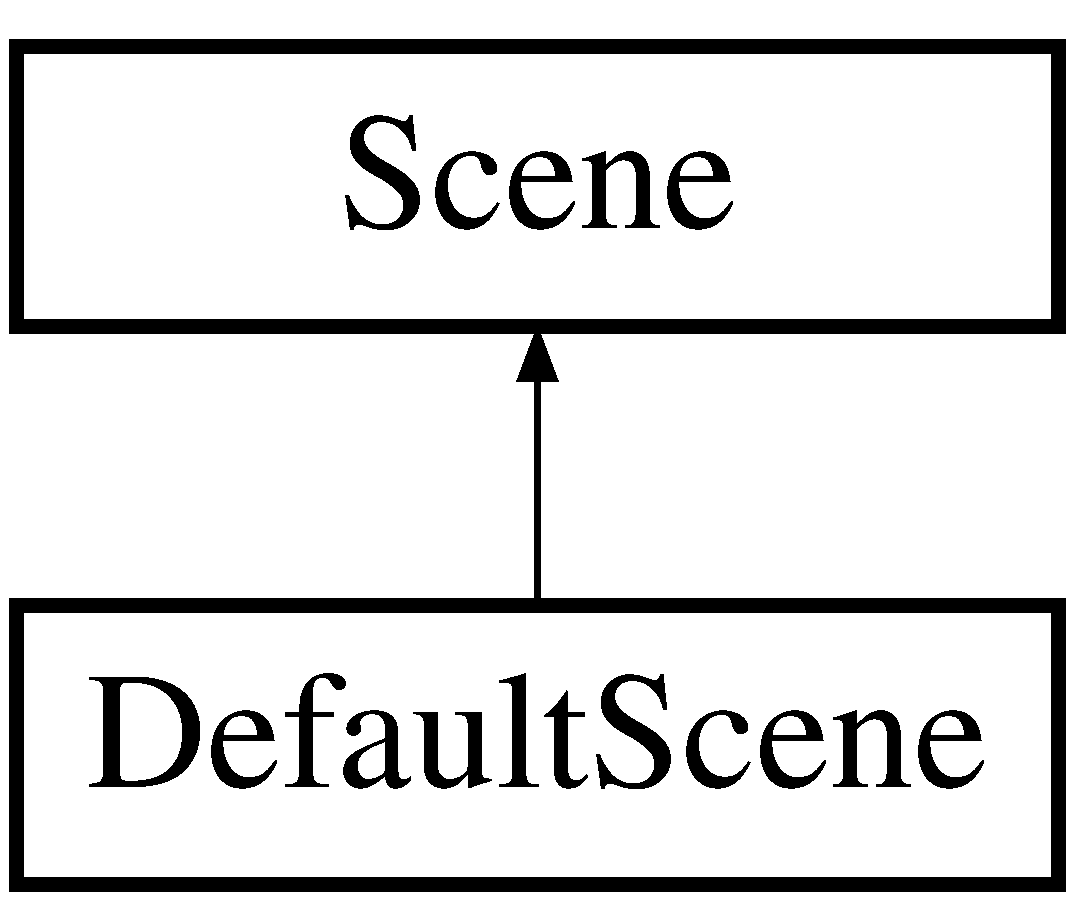
\includegraphics[height=2.000000cm]{class_scene}
\end{center}
\end{figure}
\subsection*{Public Member Functions}
\begin{DoxyCompactItemize}
\item 
\mbox{\Hypertarget{class_scene_a3b8cec2e32546713915f8c6303c951f1}\label{class_scene_a3b8cec2e32546713915f8c6303c951f1}} 
virtual \hyperlink{class_scene_a3b8cec2e32546713915f8c6303c951f1}{$\sim$\+Scene} ()
\begin{DoxyCompactList}\small\item\em Virtual destructor to allow for specific child destructor overrides. \end{DoxyCompactList}\item 
\mbox{\Hypertarget{class_scene_adcf11ea10fab6c9371fd5bfbf3d08107}\label{class_scene_adcf11ea10fab6c9371fd5bfbf3d08107}} 
virtual void \hyperlink{class_scene_adcf11ea10fab6c9371fd5bfbf3d08107}{add\+Node} (std\+::unique\+\_\+ptr$<$ \hyperlink{class_scene_node}{Scene\+Node} $>$ node)=0
\begin{DoxyCompactList}\small\item\em Adds a node to the scene graph. \end{DoxyCompactList}\item 
\mbox{\Hypertarget{class_scene_a54956adf423ce5469d3928ab26da987b}\label{class_scene_a54956adf423ce5469d3928ab26da987b}} 
virtual void \hyperlink{class_scene_a54956adf423ce5469d3928ab26da987b}{remove\+Node} (const std\+::string \&node\+Id)=0
\begin{DoxyCompactList}\small\item\em Removes a node from the scenegraph, destroying it effectively. \end{DoxyCompactList}\item 
\mbox{\Hypertarget{class_scene_a7faff47f5c1b1ebc986f768c9b9732ec}\label{class_scene_a7faff47f5c1b1ebc986f768c9b9732ec}} 
virtual void \hyperlink{class_scene_a7faff47f5c1b1ebc986f768c9b9732ec}{update} ()=0
\begin{DoxyCompactList}\small\item\em Updates the complete scene, gives all nodes a chance to update. \end{DoxyCompactList}\item 
\mbox{\Hypertarget{class_scene_a3eba6b8bf7e5be1ae0809f6f3ded3585}\label{class_scene_a3eba6b8bf7e5be1ae0809f6f3ded3585}} 
virtual void \hyperlink{class_scene_a3eba6b8bf7e5be1ae0809f6f3ded3585}{render} (\hyperlink{class_render_device}{Render\+Device} \&render\+Device)=0
\begin{DoxyCompactList}\small\item\em Renders the complete scene. \end{DoxyCompactList}\end{DoxyCompactItemize}


\subsection{Detailed Description}
A \hyperlink{class_scene}{Scene} object is the heart of the rendering in the FB renderlib. It consists of Scene\+Nodes which are the foundational objects to be rendered and the user interacts with. 

Normally, only one exists at any time, though technically, as long as you can afford it from a performance point of view, you could have multiple scenes in your program as well.

Example usage of the scene\+: 
\begin{DoxyCode}
\textcolor{comment}{// Setup phase}
\hyperlink{class_scene}{Scene} scene;
scene.\hyperlink{class_scene_adcf11ea10fab6c9371fd5bfbf3d08107}{addNode}(playerNode);
scene.\hyperlink{class_scene_adcf11ea10fab6c9371fd5bfbf3d08107}{addNode}(enemy1);
scene.\hyperlink{class_scene_adcf11ea10fab6c9371fd5bfbf3d08107}{addNode}(enemy2);

\textcolor{comment}{// in game loop}
\textcolor{keywordflow}{while} (gameRunning) \{
    scene.\hyperlink{class_scene_a7faff47f5c1b1ebc986f768c9b9732ec}{update}();
    scene.\hyperlink{class_scene_a3eba6b8bf7e5be1ae0809f6f3ded3585}{render}(myRenderDevice);
\}
\end{DoxyCode}
 

The documentation for this class was generated from the following files\+:\begin{DoxyCompactItemize}
\item 
C\+:/\+Users/martin/\+Documents/\+Visual Studio 2013/\+Projects/glfw\+\_\+test/\+Render\+Lib/scene.\+h\item 
C\+:/\+Users/martin/\+Documents/\+Visual Studio 2013/\+Projects/glfw\+\_\+test/\+Render\+Lib/scene.\+cpp\end{DoxyCompactItemize}

\hypertarget{class_scene_node}{}\section{Scene\+Node Class Reference}
\label{class_scene_node}\index{Scene\+Node@{Scene\+Node}}


A \hyperlink{class_scene_node}{Scene\+Node} is the main building block of a scene and represents the \char`\"{}game objects\char`\"{} of a game. Each \hyperlink{class_scene_node}{Scene\+Node} has a location and rotation in the world, and can update and render itself during a frame of execution.  




{\ttfamily \#include $<$scenenode.\+h$>$}

\subsection*{Public Member Functions}
\begin{DoxyCompactItemize}
\item 
\mbox{\Hypertarget{class_scene_node_ae4436f7c7d6ea817cfdce7e539f99e13}\label{class_scene_node_ae4436f7c7d6ea817cfdce7e539f99e13}} 
{\bfseries Scene\+Node} (const \hyperlink{class_scene_node}{Scene\+Node} \&other)=delete
\item 
\mbox{\Hypertarget{class_scene_node_a726714ab2af70380202fe64bb4532e04}\label{class_scene_node_a726714ab2af70380202fe64bb4532e04}} 
\hyperlink{class_scene_node}{Scene\+Node} \& {\bfseries operator=} (const \hyperlink{class_scene_node}{Scene\+Node} \&other)=delete
\item 
\mbox{\Hypertarget{class_scene_node_afed43bacb24221017fa6bb237bf1def1}\label{class_scene_node_afed43bacb24221017fa6bb237bf1def1}} 
virtual R\+E\+N\+D\+E\+R\+L\+I\+B\+\_\+\+A\+PI void {\bfseries add\+Component} (std\+::unique\+\_\+ptr$<$ \hyperlink{class_node_component}{Node\+Component} $>$ component)
\item 
\mbox{\Hypertarget{class_scene_node_a501c1c791e70537487de1354cbf313d7}\label{class_scene_node_a501c1c791e70537487de1354cbf313d7}} 
virtual R\+E\+N\+D\+E\+R\+L\+I\+B\+\_\+\+A\+PI void {\bfseries remove\+Component} (const std\+::string \&component\+Id)
\item 
\mbox{\Hypertarget{class_scene_node_a78106bd0e7daa1871dc0fb26a98c09a6}\label{class_scene_node_a78106bd0e7daa1871dc0fb26a98c09a6}} 
virtual R\+E\+N\+D\+E\+R\+L\+I\+B\+\_\+\+A\+PI void {\bfseries update} (\hyperlink{class_game_time}{Game\+Time} \&game\+Time)
\item 
\mbox{\Hypertarget{class_scene_node_a25e06dbc543062880a82246e525a9725}\label{class_scene_node_a25e06dbc543062880a82246e525a9725}} 
virtual R\+E\+N\+D\+E\+R\+L\+I\+B\+\_\+\+A\+PI void {\bfseries render} (\hyperlink{class_render_device}{Render\+Device} \&render\+Device)=0
\item 
\mbox{\Hypertarget{class_scene_node_a4a0b83e00a3edd492423970b44eb68cc}\label{class_scene_node_a4a0b83e00a3edd492423970b44eb68cc}} 
virtual R\+E\+N\+D\+E\+R\+L\+I\+B\+\_\+\+A\+PI \hyperlink{class_node_component}{Node\+Component} \& \hyperlink{class_scene_node_a4a0b83e00a3edd492423970b44eb68cc}{get\+Component} (const std\+::string \&component\+Id)
\begin{DoxyCompactList}\small\item\em Queries the node for a component with the given id. \end{DoxyCompactList}\end{DoxyCompactItemize}


\subsection{Detailed Description}
A \hyperlink{class_scene_node}{Scene\+Node} is the main building block of a scene and represents the \char`\"{}game objects\char`\"{} of a game. Each \hyperlink{class_scene_node}{Scene\+Node} has a location and rotation in the world, and can update and render itself during a frame of execution. 

Scene\+Nodes follow a modular approach in that most of its functionality is implemented through Node\+Components. A \hyperlink{class_node_component}{Node\+Component} can extend the functionality of a \hyperlink{class_scene_node}{Scene\+Node} in arbitrary ways, as its \char`\"{}execute\char`\"{} method is called once per frame, when the update method is called.

Please note, that through Node\+Components it is not possible to influence the way an object is rendered. Possibly, this constraint will be lifted in the future. 

The documentation for this class was generated from the following files\+:\begin{DoxyCompactItemize}
\item 
C\+:/\+Users/martin/\+Documents/\+Visual Studio 2013/\+Projects/glfw\+\_\+test/\+Render\+Lib/scenenode.\+h\item 
C\+:/\+Users/martin/\+Documents/\+Visual Studio 2013/\+Projects/glfw\+\_\+test/\+Render\+Lib/scenenode.\+cpp\end{DoxyCompactItemize}

\hypertarget{class_texture}{}\section{Texture Class Reference}
\label{class_texture}\index{Texture@{Texture}}


The documentation for this class was generated from the following file\+:\begin{DoxyCompactItemize}
\item 
C\+:/\+Users/martin/\+Documents/\+Visual Studio 2013/\+Projects/glfw\+\_\+test/\+Render\+Lib/texture.\+h\end{DoxyCompactItemize}

%--- End generated contents ---

% Index
\backmatter
\newpage
\phantomsection
\clearemptydoublepage
\addcontentsline{toc}{chapter}{Index}
\printindex

\end{document}
